\title{Seminarski rad}
\documentclass[12pt,a4paper]{article}
\usepackage[left=25mm, top=25mm, bottom=25mm]{geometry}
\usepackage{graphicx}
\usepackage{siunitx}

%\usepackage[T1]{fontenc}
\usepackage[utf8]{inputenc}
\usepackage[T1]{fontenc}
\usepackage{amsmath}
\usepackage{hyperref}
\hypersetup{colorlinks=true, linkcolor=black, citecolor=black, filecolor=black, urlcolor=black, pdftitle=, pdfauthor=Corporate Edition, pdfsubject=, pdfkeywords=}
\usepackage{refstyle}
\usepackage{caption}
%\newcommand\textsubscript[1]{\ensuremath{{}_{\text{#1}}}}
% List styles
\newcounter{saveenum}
\newcommand\liststyleWWNumi{%
\renewcommand\theenumi{\arabic{enumi}}
\renewcommand\theenumii{\alph{enumii}}
\renewcommand\theenumiii{\roman{enumiii}}
\renewcommand\theenumiv{\arabic{enumiv}}
\renewcommand\labelenumi{\theenumi.}
\renewcommand\labelenumii{\theenumii.}
\renewcommand\labelenumiii{\theenumiii.}
\renewcommand\labelenumiv{\theenumiv.}
}
\newcommand\liststyleWWNumii{%
\renewcommand\theenumi{\arabic{enumi}}
\renewcommand\theenumii{\alph{enumii}}
\renewcommand\theenumiii{\roman{enumiii}}
\renewcommand\theenumiv{\arabic{enumiv}}
\renewcommand\labelenumi{\theenumi.}
\renewcommand\labelenumii{\theenumii.}
\renewcommand\labelenumiii{\theenumiii.}
\renewcommand\labelenumiv{\theenumiv.}
}
\newcommand\liststyleWWNumiv{%
\renewcommand\theenumi{\arabic{enumi}}
\renewcommand\theenumii{\alph{enumii}}
\renewcommand\theenumiii{\roman{enumiii}}
\renewcommand\theenumiv{\arabic{enumiv}}
\renewcommand\labelenumi{\theenumi.}
\renewcommand\labelenumii{\theenumii.}
\renewcommand\labelenumiii{\theenumiii.}
\renewcommand\labelenumiv{\theenumiv.}
}
\newcommand\liststyleWWNumv{%
\renewcommand\theenumi{\alph{enumi}}
\renewcommand\theenumii{\alph{enumii}}
\renewcommand\theenumiii{\roman{enumiii}}
\renewcommand\theenumiv{\arabic{enumiv}}
\renewcommand\labelenumi{\theenumi)}
\renewcommand\labelenumii{\theenumii.}
\renewcommand\labelenumiii{\theenumiii.}
\renewcommand\labelenumiv{\theenumiv.}
}
\renewcommand{\figurename}{Slika}
\renewcommand\contentsname{Sadržaj}
\renewcommand\listfigurename{Sadržaj slika}

\begin{document}

\begin{titlepage}
	\begin{center}
		\vspace{1cm}
		
		\begin{figure} [h]
		\centering
		
\includegraphics{logo.png}
		\end{figure}

		

		\vspace{0.5cm}
		\large MATEMATIČKI FAKULTET\\
		\large  RAČUNARSTVO I DRUŠTVO

		\vspace{3cm}

		\textbf{SEMINARSKI RAD}

		\vspace{3cm}

		\textbf{\Huge \vspace{0.5cm} Zašto znanje ne treba da bude beslatno}

		\vfill

		\vspace{0.8cm}

		Student: Jelena Ivanović\\
		Broj indeksa: 365/19\\

		\vspace{1cm}

		Jun, 2023
	\end{center}
\end{titlepage}

\tableofcontents
\newpage
\listoffigures
\newpage
 
\section{\large{\textbf{UVOD}}}

\indent  Akademsko izdavaštvo je podvrsta izdavašta koje objavljuje naučna istraživanja i naučne radove. Veliki broj akademskih radova se izdaje u akademskim dnevnim člancima, najčešće u vidu knjiga, ali postoji i deo koji nisu formalno objavljeni, već samo odštampani ili postavljeni na internet i takav vid izdavaštva nazivamo „siva literatura“. Recenzija ili urednička ocena je jedna od bitnijih stavki kada je akademsko izdavaštvo u pitanju, po njoj se većina radova kvalifikuje i odobrava za objavljivanje.

   Ceo proces je veoma kompleksan i potrebno je puno vremena da bi pregled i recenziranje rada bilo pouzdano, zato se standardi kvaliteta i selektivnost recenzija razlikuje od izdavača do izdavača i od časopisa do časopisa. Vrste publikacija koje se prihvataju za objavljivanje da bi doprineli znanju i nauci u nekoj zemlji, razlikuju se od oblasti do oblasti. Najčešće svaka afirmisana akademska disciplina ima svoje časopise ali postoje i slučajevi kada jedan časopis posveti po jedan podeljak za svaku različitu disciplinu.
   
   Akademsko izdavaštvo prolazi kroz velike promene jer prelazi sa štampanog na elektronski format i poslovni modeli se znatno razlikuju u elektronskom okruženju. Od ranih 1990-ih, licenciranje elektronskih izvora, posebno časopisa, bilo je vrlo često. Važan trend, posebno u pogledu naučnih časopisa, je otvoreni pristup (engl. Open access), koji predstavlja slobodan, besplatan, neograničen onlajn pristup naučnim radovima, pre svega akademskim člancima, knjigama i disertacijama. Otvoreni pristup se ispoljava u dva osnovna oblika: otvorene arhive i časopise otvorenog pristupa, u potpunosti ili delimično. Zbog sve veće želje za besplatnim pristupom akademskih knjiga i časopisa dolazi do sukoba dve strane. 



\section{\large\textbf{ISTORIJAT AKADEMSKOG IZDAVAŠTVA}}

\indent 

    Komunikacija je glavni faktor za razvoj i prenošenje znanja između naučnika. Ona se najefikasnije I najpouzdanije postiže upravo preko naučnih članaka, knjiga i časopisa. Objavom i deljenjem svojih istraživanja, naučnici su mogli doprineti napretku saznanja, na koja kasnije su mogla da se nadovežu I nova saznanja.
  
   U početku se komunikacija odvijala isključivo neformalno, putem pisama i usmenih razgovora. Mane ove vrste komunikacije bile su brojne: problem analize i vrednovanja informacija, teže razmenjivanje ideja i informacija, objavljivanja rezultata, nedostupnost rezultata široj naučnoj zajednici, samim tim i manji broj kritičara i poteškoće u proveri i verifikaciji.
   
   Zbog nepraktičnosti i nedostatka neformalne komunikacije, problema vrednovanja rezultata, pokrenute su različite udružene organizacije naučnika. Cilj im je bio da promovišu i razgovaraju o prošlim, sadašnjim i budućim istraživanjima. Prvo takvo udruženje je ,,Akademia de Licei“ u Parizu, koje je funkcionisalo od 1600. do 1609. godine. Te godine objavila je zbornik rasprava sa svojih sastanaka pod nazivom ,,Gesta Lynceorum". To je najstarija publikacija koju je izdala jedna naučna zadruga. Međutim, i dalje je bio prisutan problem vrednovanja objavljenog zbog nedostatka objektivnih parametara i nedostupnosti informacija široj naučnoj zajednici. Zato je 1665. godine počeo izlaziti časopis ,,Le Journal de Scavans “, prvi akademski časopis, koji je pokrenuo Denis de Salo. Osmislio ga je Žan Batist Kobler kao instrument rukovođenja intelektualnim životom Francuske i on predstavlja jednu novu vrstu periodika, potpuno posvećenih nauci i umetnosti: „Katalog knjiga štampanih u Evropi“, kako ga predstavlja urednik u uvodnom delu. U njemu se objavljuju odlomci i sižei knjiga, nekrolozi posvećeni slavnim intelektualcima, kritike dela štampanih u raznim delovima Evrope. Potražnja za ovim časopisom bila je tolika da se ubrzo pojavio na nemačkom i italijanskom jeziku.
   
   Po uzoru na Francusku krenule su I druge zemlje da objavljuju radove. Pa tako u Engleskoj 1665. počinje izlaziti časopis ,,Filozofske transakcije" (engl. Philosophical Transactions) u izdanju Kraljevskog društva u kojem su se objavljivale naučne novosti i zapažanja. Nadalje, u Italiji 1668. godine počinje da izlazi časopis ,,Giornale de'Letterati“, a zatim profesor Oto Menke, 1682. godine u Lajpcigu štampa na latinskom jeziku “Acta Eruditorium”, u kojim Lajbnic iznosi 1684. godine „novi metod“ diferencijalnog računa. 
   
   Rani naučni časopisi prihvatili su nekoliko modela: neke je vodio jedan pojedinac koji je vršio uređivačku kontrolu nad sadržajem, često jednostavno objavljujući izvode iz pisama kolega, dok su drugi koristili proces grupnog donošenja odluka, bliže usklađen sa savremenom recenzijom. Tek sredinom 20. veka recenzije su postale standard.
   
   Devedesetih godina 20. veka pojavljuju se prve knjige u elektronskom obliku. Projekat Gutemberg koji je pokrenuo Majkl Hart je rezultirao početkom nove epohe za širenje znanja. Ovaj projekat je doživeo veliki uspeh iz razloga što su knjige bile pristupačnije, jer je svako mogao da ih “skine” bez obzira na softver i hardver koji poseduju. 
  
   Od 2006. godine gotovo svi naučni časopisi objavljuju svoju elektronsku verziju, a neki su se čak odlučili da upotpunosti pređu samo na elektronsko izdavaštvo naučnih radova. Mnoge biblioteke kupuju samo elektronski format časopisa, a papirnu verziju uzimaju samo ako je u pitanju veoma traženo i popularno delo. Zbog brzine i troškova objavljivanja dolazi do toga da može da se napravi razmak između elektronskog i uobičajenog izdavaštva i to do nekoliko meseci, zbog toga papirni časopisi postaju neidealni format za objavljivanje najnovijih istraživanja. Zato mnogi izdavači odmah objavljuju elektronsku verziju časopisa.

\begin{figure} [h]
\centering  
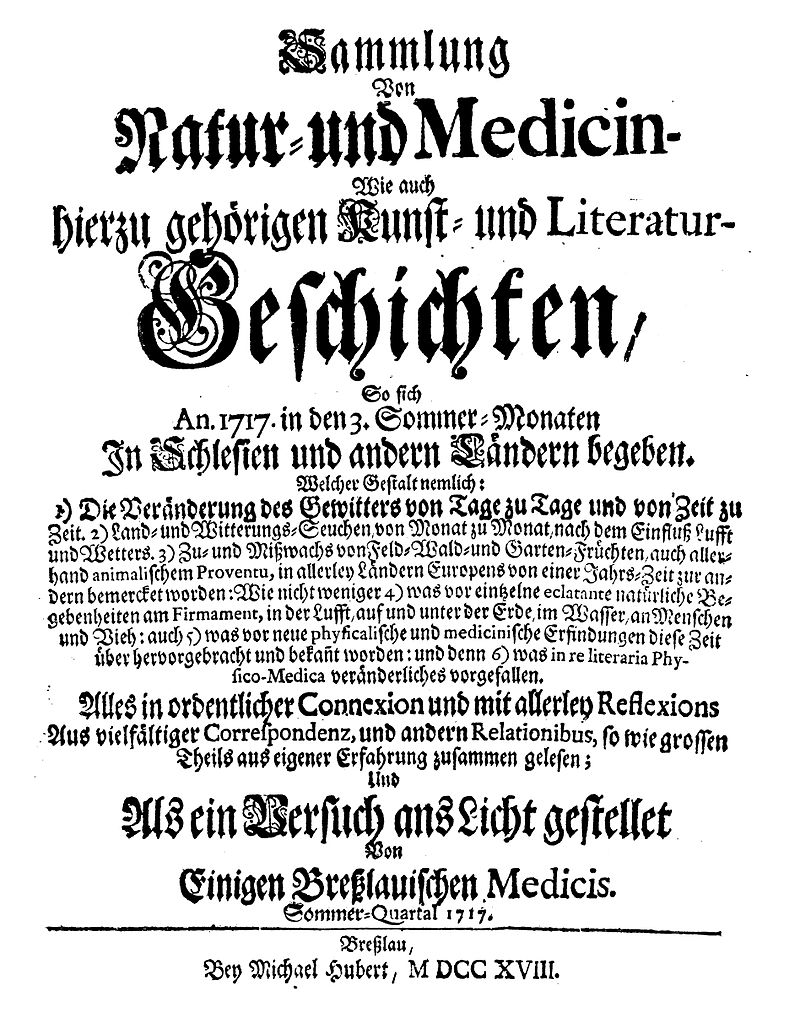
\includegraphics [width=5cm] {slika1.png} 
\caption{ Naslovnica nemačkog medicinskog časopisa iz 1718.}\label{slika1}
\end{figure}  
\newpage

\section{\large\textbf{NAUČNO BOGATSTVO ZEMLJE}}
\indent 

    Bogatstvo države predmet je konstantnog i sve većeg interesovanja ekonomista. Sa porastom značaja nauke I tehnologije u proučavanju ekonomskog razvoja, istraživačka pažnja proširena je i na naučne kapacitete zemalja. U upotrebu je uvedena sintagma "naučno bogatstvo naroda". Reč je o komparativnim istraživanjima (naučnog učinka, doprinosa, razvijenosti i, u novije vreme, efektivnosti) kojima je krajnji cilj unapređenje i racionalizacija naučne delatnosti u zemljama. Za poređenje se najčešće koriste bibliometrijski pokazatelji, zasnovani na produktivnost i citiranosti. Kao izvor obično se koriste baze podataka Instituta za naučne informacije (ISI), Filadelfija, koje su prvenstveno tome i namenjene. Na osnovu jedne takve studije utvrđeno je ono što je i bilo za očekivati, da najveću ukupni nacionalni učinak u nauci imaju SAD. Američkim autorima pripada svaki treći (tačnije \SI{34.6}{\percent}) članak i svaki drugi (\SI{49}{\percent}) citat u ISI bazama. Na drugom mestu je Velika Britanija, sa oko desetak odsto svetske produkcije. Najveći deo svetskog učinka, više od dve trećine, ostvaruju najrazvijenije zemlje Zapada.
  
   Studije ove vrste su previše skupe da bi se radile radi radoznalosti, zato postoje određeni kriterijumi po kojim se zemlje rangiraju po uspešnosti razvoja nauke.
   
   Jedan od takvih je odnos između broja objavljenih i citiranih radova (RCI, relative citation impact) koji se uzima za merilo kvaliteta radova. Prema tom indeksu SAD ostaju na prvom mestu na svetu, ali se položaj drugih zemalja menja, pa neke male dospevaju na vrh rang liste. Švajcarska je npr, druga, Švedska treća, a Danska četvrta. Istovremeno opada rang zemalja koje svoj doprinos ostvaruju više brojnošću istraživača nego obimom ulaganja u nauku (Kina, Indija). Još su korisniji pokazatelji koji uzimaju u obzir nacionalni dohodak, broj istraživača ili sredstva uložena u nauku. Oni više govore o efektivnosti nacionalne nauke, a posredno i kvalitetu organizacije naučne delatnosti. Tako je s obzirom na citiranost u odnosu na ulaganja na prvom mestu Velika Britanija, ispred SAD i Kanade. I u tom pogledu neke male evropske zemlje nadmašuju mnoge najrazvijenije. Dragocen je i pokazatelj RCA (revealed comparative advantage) iz koga se nacionalni učinak vidi disciplinarno. Analize otkrivaju da su npr. neke male evropske zemlje (Danska na prvom mestu) više nego druge u svetu usredsređene na biomedicinska istraživanja, dok neke azijske prednjače po tome koliko drže do računarstva, inženjeringa i istraživanja materijala. 

    \qquad
\begin{figure} [h]
\centering  
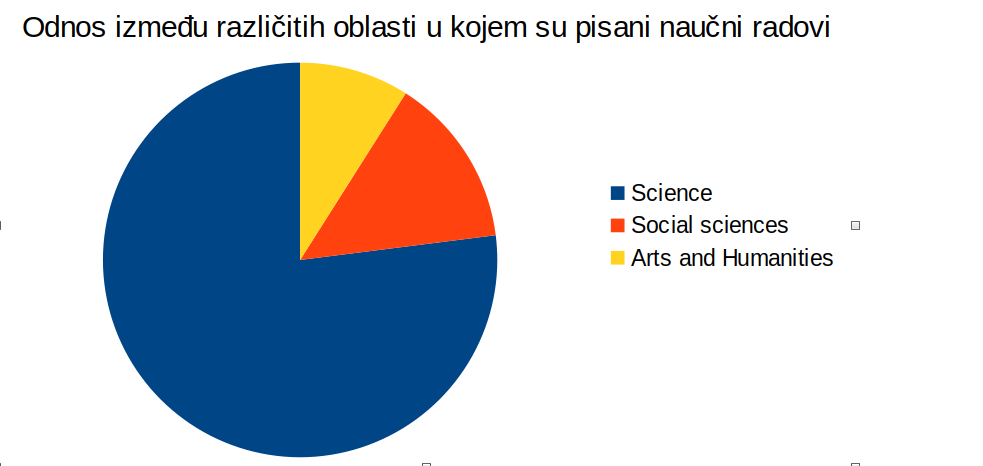
\includegraphics [width=10cm] {slika2.png} 
\caption{Statistika zastupljenosti oblasti}\label{slika2}
\end{figure}  

\newpage
\subsection{\large{\textbf{Koliko je, bibliometrijski mereno, naučno bogatstvo Srbije? }}}
\indent

  Kada se iskaže brojem radova objavljenih u SSCI časopisima i uporedno, u odnosu na zemlje iz okruženja, naš učinak u oblasti društvenih nauka je više nego skroman. U periodu 1991-1999 može se identifikovati 271 radova autora s jugoslovenskom adresom (svega tri su iz Crne Gore), od čega više od trećine otpada na manje vredne priloge (prikaze knjiga i sl.). Produktivnost naših autora na međunarodnoj sceni osetno je niža od one koju imaju njihove grčke, mađarske, bugarske, slovenačke i hrvatske kolege. U regionu naš je učinak samo iznad albanskog, BiH, i makedonskog, otprilike u nivou Rumunije, gde su društvene nauke tradicionalno u podređenom položaju. Nedovoljno je za utehu, ali treba uočiti da je kvalitet časopisa u kojima su objavljivali srpski autori, izražen impakt faktorom (IFi), ne zaostaje za drugima. Neke od zemalja koje imaju veći učinak od Srbije, na primer Slovenija, imaju višestruko manje istraživača. Neke druge, kao što su Bugarska, praktično su donedavna trpele posledice važnosti ideologije nad metodologijom. Uprkos tome bugarski istraživači iskazuju veću sposobnost istupanja na međunarodnoj sceni. Iz podataka se vidi da je napredak Hrvatske, ubedljivo najveći u regionu, presudno doprinosi okolnost da je ona u SSCI predstavljena s jednim novim časopisom (ukupno dva; Slovenija od nedavno s jednim, Srbija ni sa jednim). Na taj način autori, objavljujući u nacionalnim časopisima direktno doprinose međunarodnoj nauci i istovremeno učinku sopstvene zemlje. Za male zemlje to i jeste najbolja strategija uključivanja u međunarodnu nauku. Najbolja i zato što je najjeftinija.

    \qquad

   \begin{tabular}{|c|c|c|c|c|c|c|c|c|c|}
  \hline
    & radovi & r-d & član & kon & IF-i & lok & čl-o & IN & IF-o\\
  \hline
  SR & 271 & 269 & 177 & 0.25 & 0.60 & 0.203 & 464 & 0.377 & 0.68\\
  \hline
  HR 4 & 856 & 315 & 742 & 0.03 & 0.59 & 0.446 & 513 & 0.465 & 0.59\\
  \hline
  SL & 325 & 311 & 255 & 0.11 &0.54 & 0.404 & 305 & 0.793 & 0.51\\
  \hline
  BiH & 16 & 16 & 9 & 0.13 & 0.34 & 0.444 & 462 & 0.019 & 0.70\\
  \hline
  MK & 24 & 24 & 10 & 0.58 & 0.60 & 0.800 & 123 & 0.081 & 0.64\\
  \hline
  RU & 193 & 193 & 122 & 0.28 & 0.43 & 0.451 & 441 & 0.276 & 0.50\\
  \hline
  AL & 24 & 24 & 19 & 0.04 & 0.51 & 1 & 222 & 0.086 & 0.52\\
  \hline
  GR & 1696 & 1696 & 1403 & 0.07 & 0.62 & 0.376 & 1323 & 1.056 & 0.59\\
  \hline
  BU & 421 & 416 & 301 & 0.18 & 0.66 & 0.389 & 473 & 0.626 & 0.48\\
  \hline

    
  \hline
  
\end{tabular}

    \qquad

    
    radovi = ukupan broj objavljenih radova; r-d= ukupan broj objavljenih radova van domaćih časopisa referisanih u SSCI; član = broj članaka; kon = proporcija kongresnih apstrakata; IFi = prosečan impakt faktor časopisa u kojima su objavljeni članci iz zemlje; lok = proporcija radova na lokalne/nacionalne teme; čl-o = broj članaka autora izvan regiona koji se tiču zemlje; IN = indeks eksterne nezavisnosti; IFo = prosečan impakt faktor časopisa u kojima su objavljeni članci o zemlji 

    \qquad
      Domaći autori najviše su objavljivali u SSCI časopisima iz oblasti psihologije. Zatim su po brojnosti radovi iz ekonomije, političkih nauka i međunarodnih odnosa, dok ih je najmanje, tačnije nijedan, iz filozofije, pedagogije, defektologije, demografije, istorije, geografije, finansija i još nekoliko užih disciplina. Naš učinak je nulti i u modernim disciplinama, na primer javnoj administraciji i poslovnim informacijama. Zanimljivo je da nemamo radova ni u oblasti etničkih studija. To je u potpunom neskladu s publicističkom (hiper)aktivnošću pravnika u zemlji. Ukupan broj disciplina u kojima nemamo nijedan rad iznosi 18 (od 51) i veći je nego u drugim zemljama iz regiona, izuzimajući Rumuniju i zemlje s kojima je poređenje neumesno, dakle, Albaniju, BiH i Makedoniju. 


    \section{\large\textbf{ZNAČAJNOST NAUČNIH ČASOPISA}}
    \indent
    
     Naučni časopisi su centralne institucije nauke. To nisu akademije nauka, univerziteti ili naučna udruženja. Stanje stvari u jednom domenu nauke, ono što je trenutno bitno ili važeće, ne traži se u naučnim enciklopedijama niti u udžbenicima, već u člancima objavljenim u časopisima. Časopisi su neke vrste službeni listovi u kojima se oglašavaju sadržaji aktuelnog naučnog saznanja , novog članka kojim se to saznanje upotpunjuje ili potire. 
   
    Publikovanje radova u međunarodnim naučnim časopisima jeste način naučne komunikacije i ključni pokazatelj kompetentnosti naučnog i nastavnog kadra. Publikovanjem novoostvoreni naučni rezultat postaje vidljiv i podložan proveri u naučnoj javnosti. To je prvi korak ka legitimnom uvođenju novog naučnog rezultata u skup postojećih naučnih znanja. Proces publikovanja naučnih radova u međunarodnim naučnim časopisima je dugotrajan, neizvestan i zahtevan. Nivo prihvatanja radova u nekim vodećim svetskim naučnim časopisima predstavlja deset procenata od broja podnetih radova što je posledica visokih kriterijuma, a pre svega kriterijuma relevantnosti i originalnosti. 
    \qquad

     Svrha rada je: 
    \begin{itemize}
        \item isticanje važnosti izrade naučnih dela međunarodnog značaja kao kritičnog elementa naučne kompetentnosti nastavno-naučnog kadra
        \item prikaz metodologije pripreme radova i čitavog postupka do njihovog publikovanja i motivacija akademske zajednice za aktivnosti publikovanja radova u međunarodnim naučnim časopisima.
        \item Izloženi sadržaji zasnovani su na originalnom praktičnom iskustvu publikovanja radova za jedan vrhunski međunarodni naučni časopis.
    \end{itemize}    
    \qquad 

    Autoritet časopisa ima više izvora, ali je svakako najvažniji visok stepen verifikacije sadržaja. U časopisima on je najviši mogući. Jedino tu mehanizam za verifikaciju obuhvata ukupnu naučnu javnost, od urednika, preko recenzenata, do svih pripadnika naučne zajednice kao potencijalnih kritičara. Kvalitet vrhunskih časopisa meri se sistematskim praćenjem njihove uticajnosti. Zato vrhunski naučni časopisi imaju tako razrađen postupak prihvatanja radova, tako ugledne urednike i recenzente, tako visoku cenu i tako dugu tradiciju. 

        
            
        \begin{figure} [h]
        \centering  
        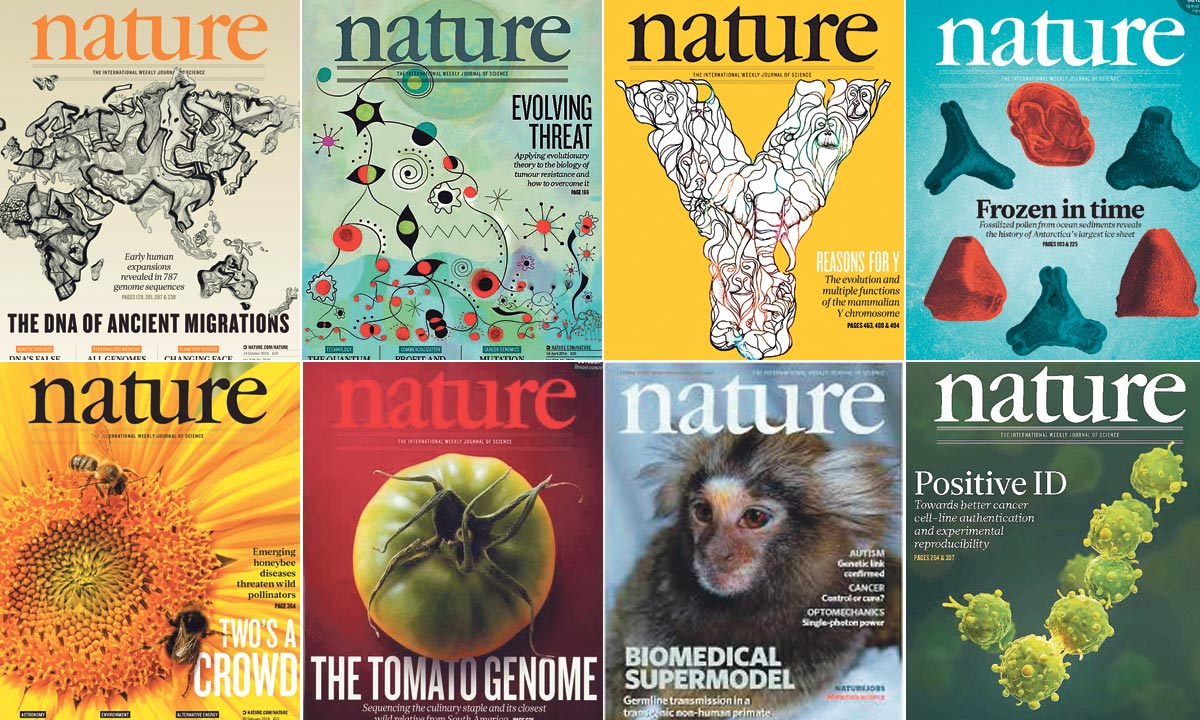
\includegraphics [width=10cm] {nature.png} 
        \caption{"Nature"- najznačajniji naučni časopis na svetu}\label{slika2}
        \end{figure}  


     U nerazvijenim sredinama značaj naučnih časopisa, se ne razume. Kod nas je na delu to da se časopisi podržavaju retorički, a sabotiraju finansijski. Takav odnos ima za posledicu to da nijedan naš časopis nije predstavljen u citatnim bazama ISI. Samim tim ne može se braniti važeća kategorizacija MNTR koja status časopisa međunarodnog značaja priznaje mnogima. Činjenica da su neki domaći časopisi referisani u nekim disciplinarnim međunarodnim sekundarnim publikacijama, odnosno bazama, pohvalna je ali nedovoljna za takvu kvalifikaciju. Mera međunarodnog značaja može biti samo citiranost (impakt) časopisa, a dokaz njegovog postojanja samo svrstavanje časopisa u neku od baza ISI. 
     
     Slab međunarodni učinak ne mora biti posledica slabog kvaliteta. Bar deo naših radova ima šta da ponudi međunarodnoj naučnoj javnosti. Problem je u tome što naši časopisi nisu dovoljno “vidljivi”.
     
     Pored toga, publikovanje radova u međunarodnim naučnim časopisima najslabija je karika u sistemu nastavnih i naučnih institucija u Ministarstvu odbrane Republike Srbije. U našoj praksi nastavnog i naučnog rada taj proces nije dovoljno poznat, niti je u potrebnoj meri priznat, a često je praćen nekim pogrešnim predrasudama. 
     

\section{\large\textbf{POJAVA TRAŽNJE ZA OTVORENOM NAUKOM}}
\indent 

Tokom protekle dve decenije, naučno izdavaštvo je doživelo pravu revoluciju, koju je omogućila pojava World Wide Web-a. Ova revolucija sadrži dve povezane faze.

   Prva faza je prelazak sa samo štampanih časopisa na paralelno štampano I elektronsko izdavanje. Krajem 20. veka naučnici su skoro sva svoja čitanja obavljali iz papirnih izdanja, dobijenih kao lične kopije, kružeći samo unutar njihovih organizacija ili preuzimajući brojeve iz biblioteka.
   
   Danas međutim vlada režim preuzimanja digitalne kopije ili čitanje direktno sa ekrana. Zbog toga jedan prosečan istraživač na univerzitetu ima pristup mogo širem spektru članaka iz časopisa nego ikada ranije tokom ere štampanja.
   
   Druga faza u ovoj revoluciji je pristup člancima bez ikakvih ograničenja koja postavljaju pretplate na časopise. Otvoreni pristup se pojavio u ranim 90-tim, pokrenut mogućnostima koje nudi veb, ali I delimično zbog činjenice da su pretplate brže rasle nego sama stopa inflacije. 
   
   Kriza u akademskom izdavaštvu je očigledna jer je povezana sa kombinovanim pritiskom smanjenja budžeta na univerzitetima i povećanim troškovima časopisa (kriza serijskih publikacija). Smanjenje univerzitetskog budžeta smanjilo je budžete biblioteka i subvencije izdavačima povezanim sa univerzitetima. Na humanističke nauke posebno je uticao pritisak na univerzitetske izdavače koji su imali manju mogućnost da objavljuju monografije kada biblioteke ne mogu da priušte da ih kupe.
   
   Na primer, Udruženje istraživačkih biblioteka je otkrilo da su 1986. godine biblioteke potrošile \SI{44}{\percent} svog budžeta na knjige u poređenju sa  \SI{56}{\percent} na časopise; dvanaest godina kasnije, taj odnos je promenjen na  \SI{28}{\percent} i  \SI{72}{\percent}“. U međuvremenu se sve češće očekuju monografije u humanističkim naukama. 2002. godine Udruženje modernih jezika izrazilo je nadu da će elektronsko objavljivanje rešiti problem.
   
   U ranim danima većina časopisa otvorenog pristupa bili su male pojedinačne organizacije koje su vodile grupe ili pojedinačni naučnici. Nakon 2000. godine pojavio se sve veći broj profesionalnih izdavača otvorenog pristupa (npr. BioMedCentral, Public Library of Science, Hindawi, Bentham Open). Ovi izdavači obično finansiraju svoje poslovanje putem troškova objavljivanja koje naplaćuju autorima tih članaka. Oni su preokrenuli poslovni model tako što su autore napravili svojim klijentima. 
   
   Ova činjenica i promena dovela je do dileme: ko stvarno treba da finansira akademsko izdavaštvo? 



    \section{\large\textbf{ZAŠTO NAUKA NE TREBA BITI BESPLATNA}}
    \indent
     Razne studije pokazale su da je potražnja za istraživanjima otvorenog pristupa takva da su slobodno dostupni članci dosledno imali faktore uticaja koji su bili veći od članaka objavljenih pod ograničenim pristupom.
  
     Međutim, ljudi su izneli različite argumente protiv otvorenog pristupa, kako bi se zadržala određena ekskluzivnost u nauci, poput sledećih:

     \begin{itemize}
         \item mnogo nekategorizivanih informacija opterećuje naučnike
         \item nauka može da se zloupotrebljava
         \item javnost može pogrešno da tumači naučne podatke
         \item povećanje opsega nauke može da oteža verifikaciju bilo kog otkrića
         \item razlučivanje kvalitetnih rezultata od manje kvalitetnih ili nekvalitetnih, originalnih od plagijata i sl. postalo je ozbiljan problem a tehnike procene vrednosti informacija veoma zna čajne za dalji razvoj nauke.
         \item izdavači više nemaju monopol na internetu, sada je mogu će da autori sami postave materijale koje žele bez ikakve recenzije.
         \item gubitak motivacije u pisanju naučnih radova bez finansijske pomoći
         
     \end{itemize}

    \qquad
     Naučni časopisi su tu da bi se ovi problemi sprečili. Za bilo koje dobro delo potrebne su finansije kako bi ono bilo što pouzdanije i kvalitetnije. Ako se sve prepusti otvorenoj nauci internet će biti prebukiran delima mnogih ljudi, koja mogu da budu neprikladna i lažna. Naučni časopisi nam garantuju pouzdane podatke jer iza njega stoje stručno obrazovani ljudi, recezenti.
     
   Recenziranje je kamen temeljac u procesu objavljivanja naučnih radova, ali i često zanemaren faktor razvoja celokupne nauke. Zasnovano je na ideji da se rezultati svakog naučnog istraživanja moraju stručno oceniti od strane eksperata – recenzenata, pre nego se prezentuju naučnoj zajednici i javnosti. Drugim rečima, s obzirom da naučni rezultati efektivno „ne postoje“ sve dok nisu u pisanoj formi objavljeni u naučnom časopisu, sumnje i komentari izraženi od strane recenzenata zauzimaju važno mesto u celokupnom naučnom procesu. Pored toga, odobrenje recenzenata da se naučne informacije objave i razmene je jedan od najsnažnijih izraza profesionalnog priznanja pojedinaca/grupe i instrument društvene kontrole u naučnoj zajednici. Zbog izuzetnog značaja recenziranja za razvoj nauke i društvo uopšte, od recenzenata se očekuje da budu kompetentni, eksperti u odgovarajućoj oblasti i da poseduju dovoljno znanja i iskustva da procene da li su u opisanom istraživanju korišćene prikladne metode i/ili eksperimenti, da li su dobijeni rezultati tačni i pouzdani, a interpretacija rezultata razumna i zasnovana na postojećim znanjima.  
  
   Ceo proces pisanja i uređivanja naučnih radova je kompleksan i zahteva puno vremena. Razvoj nauke je veoma bitan za sam razvoj zemlje, što su veće finansije to je zainteresovanost i brzina izrade znatno veća. Pored pojedinaca koje u svoje svrhe žele da koriste naučne časopise i sama država treba da učestvuje u ulaganje u nauku. Za što bolje radove potrebni su i eksperimenti i dodatna istraživanja, što sve traži neki vid finansija. 


   
\section{\large\textbf{ZAKLJUČAK}}
\indent

    Za mlade istraživače početnike pisanje i uređivanje znanstveno-stručnih članaka za objavljivanje u međunarodnim znanstvenim časopisima težak je zadatak. Potrebno je imati znanja o tačnim metodama znanstvene obrade raspoloživih dokaza, strukturiranju znanstvenog teksta, pravilnoj strukturi teksta i o uređivanju tablica i slika. Svaki članak rezultat je multidisciplinarnog i multi-autorskog rada koji podržavaju i/ili financiraju javne ili profesionalne institucije, farmaceutske industrije ili druge organizacije veoma zainteresirane za objavljivanje, distribuciju, arhiviranje i promicanje opisanih informacija.
    Istraživačke i akademske institucije u svetu ocenjuju stupanj kvaliteta odabrane visokoškolske institucije prema kvantitetiu publiciranih znanstvenih i stručnih članaka. S obzirom na kompleksnost znanstvenog pisanja, znanstvenici koji imaju potrebna znanja i veštine u publiciranju, u svom profesionalnom području, često prema mladim autorima nastupaju kao urednici časopisa te pri pisanju članaka znatno pomažu znanstvenicima-početnicima. Opisana vrsta pomoći posebno je važna u zemljama ne-engleskog govornog područja, gdje nastojanja nekolicine entuzijastičnih glavnih urednika specijalističkih znanstvenih časopisa mogu sprečiti višekratna odbijanja rukopisa mladih autora u međunarodnim časopisima te se materijalizirati u više desetaka publiciranih članaka poboljšanjem stepena veštine pisanja i povećanjem izgleda za uvrštavanje domaćih časopisa u prestižne biomedicinske baze podataka. Mladi autori postižu izvrsne rezultate kada rade u istraživačkim institucijama te im je omogućena saradnja s stručnjacima u statistici, urednicima časopisa i stručnjacima u oblasti nauke za koju se interesuju. Da bi ovaj proces bio što uspešniji i što više mladih ljudi se zainteresovalo, potrebne su finansijske pomoći. Takođe kupovina magazina pomaže I u statističkom istraživanju, odnosno stepen zainteresovanosti čitalaca za odredjenu oblast nauke. Ljudi svoje živote posvete istraživanjima i oplenjivanjem društva, to bi trebalo da se ceni i nagradi.

\newpage
\section{LITERATURA}

    [1] Zoran V. Popović \url{http://www.solid.phy.bg.ac.rs/publications/knjiga-popovic.pdf}\\
    \quad
    [2] \url{https://kobson.nb.rs/upload/documents/oNamaPredavanja/PR2008Seminar4casVrednovanjeICitaneBazePodataka.pdf}\\
    \quad
    [3] \url{https://scindeks.ceon.rs/article.aspx?artid=0042-84261001009N}\\
    \quad
    [4] \url{https://sr.wikipedia.org/wiki/Nau%C4%8Dni_%C4%8Dasopis#Cena}\\
    \quad
    [5] \url{https://journals.plos.org/plosone/article?id=10.1371/journal.pone.0011273}\\
    \quad
    [6] \url {https://files.eric.ed.gov/fulltext/EJ837278.pdf}\\
    \quad
    [7] \url {https://www.researchgate.net/profile/Pero-Sipka/publication/216730024_Nauka_u_Srbiji_u_susret_evaluativnoj_drzavi/links/549b1ad00cf2b8037137191f/Nauka-u-Srbiji-u-susret-evaluativnoj-drzavi.pdf}\\
    \quad
    [8]\url{http://ebooks.ien.bg.ac.rs/1325/1/banovic%2C%20djukic%2C%20mitic.pdf}\\
    \quad
    [9]\url{https://hrcak.srce.hr/file/202502}\\
 \
\end{document}
